%%%%%%%%%%%%%%%%%%%%%%%%%%%%%%%%%%%%%%%%%%%%%%%%%%%%%%%%%%%%%%%%%%%%%%%%%%%%%%%%
% Template for TISMIR Papers
% 2017 version, based on previous ISMIR conference template
%%%%%%%%%%%%%%%%%%%%%%%%%%%%%%%%%%%%%%%%%%%%%%%%%%%%%%%%%%%%%%%%%%%%%%%%%%%%%%%%

\documentclass{article}

%%%%%%%%%%%%%%%%%%%%%%%%%%%%%%%%%%%%%%%%%%%%%%%%%%%%%%%%%%%%%%%%%%%%%%%%%%%%%%%%
% Sample Document LaTeX packages
%%%%%%%%%%%%%%%%%%%%%%%%%%%%%%%%%%%%%%%%%%%%%%%%%%%%%%%%%%%%%%%%%%%%%%%%%%%%%%%%

\usepackage[utf8]{inputenc}
\usepackage{tismir}
\usepackage{amsmath}
\usepackage{hyperref}
\usepackage{url}
\usepackage{graphicx}
\usepackage{booktabs}
\usepackage{lipsum}

\DeclareMathOperator*{\argmaxA}{arg\,max}

%%%%%%%%%%%%%%%%%%%%%%%%%%%%%%%%%%%%%%%%%%%%%%%%%%%%%%%%%%%%%%%%%%%%%%%%%%%%%%%%
% Title and Author information
%%%%%%%%%%%%%%%%%%%%%%%%%%%%%%%%%%%%%%%%%%%%%%%%%%%%%%%%%%%%%%%%%%%%%%%%%%%%%%%%

\title{Musical Note and Instrument Family Identification using the Constant-Q Transform}
%
\author{%
Saul Ivan Rivas Vega\thanks{Universidad Autónoma de México, IIMAS, Mexico City}%,
%~Second Author2\thanks{Research Institute Two, Campus Rd. 4, 12345 Flatland},%
%~and Third Author3\protect\footnotemark[1]
}

\date{}

%%%%%%%%%%%%%%%%%%%%%%%%%%%%%%%%%%%%%%%%%%%%%%%%%%%%%%%%%%%%%%%%%%%%%%%%%%%%%%%%
% Additional Paper Information
%%%%%%%%%%%%%%%%%%%%%%%%%%%%%%%%%%%%%%%%%%%%%%%%%%%%%%%%%%%%%%%%%%%%%%%%%%%%%%%%

% Article Type - Uncomment and modify, if necessary.
% Accepted values: research, overview, and dataset
\type{overview}

% Citation in First Page
%
% "Mandatory" (if missing will print the complete list of authors,
% including the \thanks symbols)
\authorref{Saul Ivan Rivas Vega}
%
% (Optional)
% \journalyear{2017}
% \journalvolume{V}
% \journalissue{N}
% \journalpages{xx--xx}
% \doi{xx.xxxx/xxxx.xx}

% Remaining Pages (Optional)
%
\authorshort{Saul Ivan Rivas Vega} %or, e.g., \authorshort{Author1 et al}
% \titleshort{Template for TISMIR}

%%%%%%%%%%%%%%%%%%%%%%%%%%%%%%%%%%%%%%%%%%%%%%%%%%%%%%%%%%%%%%%%%%%%%%%%%%%%%%%%
% Document Content
%%%%%%%%%%%%%%%%%%%%%%%%%%%%%%%%%%%%%%%%%%%%%%%%%%%%%%%%%%%%%%%%%%%%%%%%%%%%%%%%

\begin{document}

%%%%%%%%%%%%%%%%%%%%%%%%%%%%%%%%%%%%%%%%%%%%%%%%%%%%%%%%%%%%%%%%%%%%%%%%%%%%%%%%
% Abstract
%%%%%%%%%%%%%%%%%%%%%%%%%%%%%%%%%%%%%%%%%%%%%%%%%%%%%%%%%%%%%%%%%%%%%%%%%%%%%%%%

\twocolumn[{%
%
\maketitleblock
%
\begin{abstract}
In this paper a Naive Bayes Classifier is trained using the Constant-Q Transform coefficients as features. The use of a modern dataset and just the frequency domain features is intended for testing the robustness of these features that can then be of use for applications which perform Musical Instrument Identification and Automatic Music Transcription. The results shows a significantly high accuracy in the train/test split of the dataset and in a further testing with monophonic recordings from two music production applications.
\end{abstract}
%
\begin{keywords}
Pitch Detection; Timbre Estimation; Music Information Retrieval; Constant-Q transform; Naive Bayes
\end{keywords}
}]
\saythanks{}

%%%%%%%%%%%%%%%%%%%%%%%%%%%%%%%%%%%%%%%%%%%%%%%%%%%%%%%%%%%%%%%%%%%%%%%%%%%%%%%%
% Main Content Start
%%%%%%%%%%%%%%%%%%%%%%%%%%%%%%%%%%%%%%%%%%%%%%%%%%%%%%%%%%%%%%%%%%%%%%%%%%%%%%%%

\section{Introduction}\label{sec:introduction}
Tasks like Music Instrument Identification and Automatic Music Transcription have been widely studied within Music Information Retrieval (MIR) tasks ~\citep{Kitahara2005InstrumentII,Salamon2012MelodyEF,Gururani2019AnAM}, refer to~\citep{benetos_automatic_2013,benetos_automatic_2019} for a more extensive overview.  Being able to tackle these tasks can have a great impact on how we teach, experience and play music. Open Source implementations of such works can be found in GitHub repositories made by the authors, developers\endnote{Sevag Hanssian's repository with a compilation of pitch detection methods: \\
	\url{https://github.com/sevagh/pitch-detection}} and in full development libraries like ESSENTIA~\cite{bogdanov_essentia_2013} or Librosa~\cite{brian_mcfee-proc-scipy-2015}. 

Musical notes are named pitches, like A4, C3 and G\#2. In~\cite{schnupp_auditory_2011} pitch is defined as a subjective percept of sounds not a physical property of them. That is, pitch is how we perceive a certain sound and it could not be measurable by the sound only. Regardless, we know that periodicity in sound plays a heavy role in our perception. We measure the periodicity in a sound signal by counting how many repetitions of the period are in 1 second (Hertz). This quantification of periodicity is called "fundamental frequency" (f0). Pitch is often used interchangeably with f0, and although f0 can used to measure pitch it does not necessarily correspond to the same. Sounds we perceive with a high pitch normally have a high f0 and vice versa. Thus the complexity of pitch as subjective is often neglected outside psycho-acoustical studies.

As for musical instrument identification or recognition we can view them as sound sources and to differentiate them we now have to talk about timbre. Timbre like pitch is a subjective percept of sound which also is neglected as subjective by assuming certain properties of sound as its physical correlates. Timbre is specially distinct of pitch as for how well is defined using physical properties. In~\cite{siedenburg_timbre_2019} a review of many definitions is made and mainly discussing the one provided by the American National
Standards Institute (ANSI): "That attribute of auditory sensation which enables a listener to judge that two nonidentical sounds, similarly presented and having the same loudness and pitch, are dissimilar."
In their discussion they mention of timbre correlating with multidimensional set of sound properties varying in scale which is yet to be defined at it fullest if possible due to the context dependent results many studies have found.

The physical properties associated with timbre often used are the temporal envelope of the sound, spectral and cepstral analysis, which is the envelope of the frequency spectrum of the signal, to mention a few.
From the most used properties we find the frequency analysis and as stated in~\cite{brown_calculation_1991}:
"The frequencies that have been chosen to make up the scale of Western music are geometrically spaced. Thus the discrete Fourier transform (DFT), although extremely efficient in the fast Fourier transform implementation, yields components which do not map efficiently to musical frequencies."
The constant-Q transform is different to the DFT in which there is no constant difference between frequencies but a constant ratio of difference. The frequencies in the music scale are spaced by multiples of its fundamental frequency thus a matching constant-Q transform is equivalent to a 1/24-oct filter bank.

\section{Related Work}\label{sec:footnotes}

An overview as the one in~\cite{gerhard_pitch_2003} or ~\cite{drugman_traditional_2018} has the most common evaluation and classification of pitch estimation and audio analysis methods in general. The features extracted can be of the frequency domain, time domain or calculating special features like the Mel-frequency cepstral coefficients (MFCCs) in ~\cite{rao_pitch_2017} or using the Constant-Q Transform in  ~\cite{argenti_automatic_2011}. For timbre estimation the computational research has addressed it as part of a better defined task, being it of the musical instrument identification. The overviews ~\cite{herrera-boyer_automatic_2006,hall_study_2012} also consider features in the time and frequency domains, but differing of the previously discussed in the addressing of the multidimensionality of timbre, and specifying how the task can be performed in isolated sounds and in pitched instruments (refer to ~\cite{fuhrmann_automatic_nodate} for a review considering a broader experimental settings apart of just pitched instruments). A work making a review of MIR toolboxes is ~\cite{muller_fmp_2019} having a comprehensive and bread overview of the capabilities of such packages in a educational context. The presented approach differs in to test the robustness of the Constant-Q transform as a timbral and pitch physical correlate and descriptor in a more traditional machine learning fashion. 
\section{Model}\label{sec:proposedmodel}
The model is a Na\"{i}ve Bayes Classifier trained using the NSynth dataset~\cite{engel_neural_2017}. The dataset consists in 305,979 monophonic 16kHz audio snippets recorded from acoustic, electronic and synthesized instruments. It is organized by instrument family (Bass, Brass, Flute, Guitar, Keyboard, Mallet, Organ, Reed, String, Synth Lead, Vocal) covering every pitch of a standard MIDI piano (21-108) in five different velocities (25, 50, 75, 100, 127).
Not all instruments are capable to produce some pitches and just as a proof of concept it is not necessary to cover all of them. A subset consisting of 1554 audio snippets was used. Where there are 14 acoustic instruments per each of the 3 selected families (string, guitar, brass) with a constant velocity of 127 and the 37 pitches in the range of C1 and C4. Later the Constant-Q transformation is calculated using the implementation in Librosa~\cite{brian_mcfee-proc-scipy-2015} based on~\cite{schoerkhuber_constant-q_2010} obtaining the coefficients per frame of the audio snippets corresponding to the range from C1 to B7 (84 pitches) as shown in figure~\ref{ExampleConstantQ}. Only the coefficients of the first 16 frames are used as features for the Classifier.
\begin{figure}[h!]
	\begin{center}
	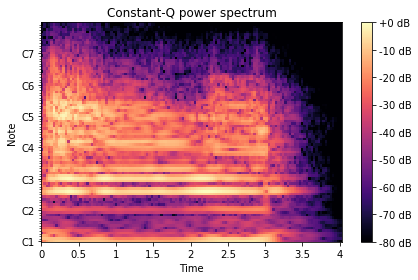
\includegraphics[scale=0.5]{ExampleConstantQ}
	\caption{Example of the spectrum of the constant-Q transform of a C1 played in a brass acoustic instrument.}
	\label{ExampleConstantQ}
	\end{center}
\end{figure}
\begin{equation}\label{eq_1}
Y \leftarrow \argmaxA_{y_k} P(Y = y_k)\prod_{i}^{d}{P(X_i|Y = y_k)}
\end{equation}
In equation~\ref{eq_1} the Constant-Q coefficients are the feature vector X with length $d=84$
 assuming a Gaussian Distribution for the values of energy on each one as in the following equation:
 \begin{equation}\label{eq_2}
 \begin{split}
 \mathcal{N}(X_i;\mu;\sigma^2) =& \frac{1}{\sqrt{2\pi\sigma^2}}e^{\frac{-(X_i - \mu)^2}{2\sigma^2}}
 \end{split}
 \end{equation}
 Parameters $\mu$ and $\sigma$ are estimated following:
 \begin{equation}\label{eq_3}
 \begin{split}
 \hat{\mu}&=\frac{1}{n}\sum_{i=1}^{n}{X_i}\\
 \hat{\sigma}^2_F&=\frac{1}{n}\sum_{i=1}^{n}{(X_i - \hat{\mu})^2}\\
 \end{split}
 \end{equation}
 Where $n$ are the number of samples in the data. The total samples are 24864, 16 frames per pitch, 37 pitches per instrument, 14 instruments per family, with 3 families. We also assume a Categorical Distribution on the pitch and instrument paired label $y_k$, which only consist of dividing the number of samples with such label by the number of total samples. From the total samples 224 correspond for each of the categories, being the 37 pitches for each of the 3 families.

\section{Evaluation}\label{sec:evaluation}
The model is to be evaluated by running experiments in a K-fold cross validation setting reporting its accuracy overall in the train/test splits of the dataset and a more empirical evaluation of composed monophonic song excerpts. 
\subsection{Experimental Setup}
The experiments consist in making 10 repetitions of a stratified K-fold cross validation of 7 partitions to calculate the average of accuracy in the model. In the train/validation split 32 samples will be for validation and 192 for training. Also all the 32 validation samples will be from instrument sources not present in the training split. That is from the 14 instrument sources for each family-pitch paired label 12 will be for training and 2 for validation. The accuracy of the model is reported and a more empirical test with custom recordings as well.

\subsection{Experimental Results}
The model showed an overall accuracy of \textbf{93.64\%} in the training data and \textbf{88.616\%} in the test data.

These results encouraged the evaluation of more general environments. The dataset was sampled by the magenta team in Google but to actually assume these results we must use these exact samples to compose songs. Although possible, many music production software as GarageBand\endnote{GarageBand for iOS, \url{https://www.apple.com/ios/garageband/}} and Ableton Live 10 Lite\endnote{Ableton Live 10 Lite, \url{https://www.ableton.com/en/products/live-lite/}} Live include already sampled instruments in the families we used in this paper. So I extended the evaluation to include 6 compositions using a sampled French Horn for Brass Family, a String Ensemble for String Family and a Nylon Concert Guitar for Guitar Family in GarageBand and a Tenor Trombone for Brass Family, a Cello for String Family and a Nylon Concert Guitar for Guitar Family in Ableton Live 10 Lite using the BBC Symphony Orchestra Discover Plug-in\endnote{BBC Symphony Orchestra Discover, \url{https://www.spitfireaudio.com/shop/a-z/bbc-symphony-orchestra-discover/}}.


The score is the same for each composition and can be seen in figure~\ref{FurtherTestingScore}. Also the constant-Q Spectral plots for each composition are in figures~\ref{ConstantQCompositions} and~\ref{ConstantQCompositions2}.
\begin{figure}[h!]
	\begin{center}
		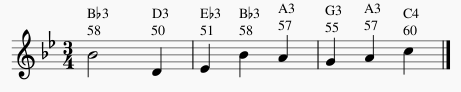
\includegraphics[scale=0.67]{FurtherTestingScore}
		\caption{Score used for further testing, the note names and MIDI-pitch numbers are shown.}
		\label{FurtherTestingScore}
	\end{center}
\end{figure}\\
\begin{figure}[h!]
	\begin{center}
		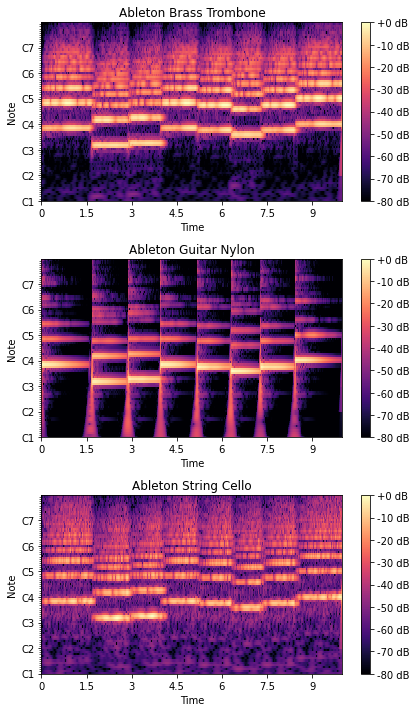
\includegraphics[scale=0.6]{download}
		\caption{Constant-Q plot of the 3 instrument families composed in Ableton Live 10 Lite, from top to bottom: Trombone (Brass), Nylon Guitar (Guitar), Cello (String).}
		\label{ConstantQCompositions}
	\end{center}
\end{figure}\\
\begin{figure}[h!]
	\begin{center}
		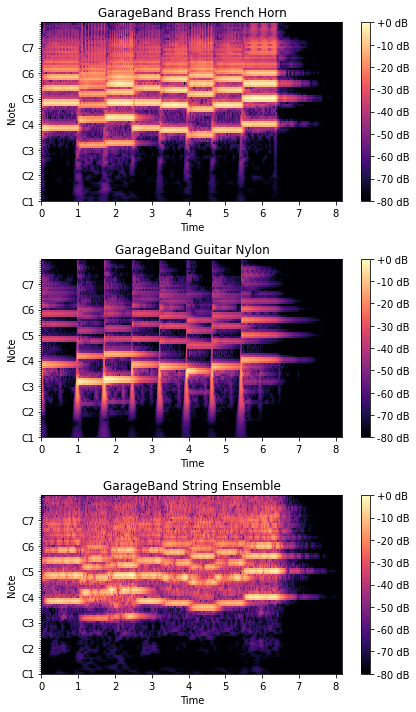
\includegraphics[scale=0.59]{download2}
		\caption{Constant-Q plot of the 3 instrument families composed in GarageBand, from top to bottom: French Horn (Brass), Nylon Guitar (Guitar), String Ensemble (String).}
		\label{ConstantQCompositions2}
	\end{center}
\end{figure}
The empirical results point that the system is able to identify the family and note quite precisely having almost all the notes of the score. But more interestingly within the sustain of a note there are some variations on its estimations. In the Guitar recordings it reported some parts as being of a string family instrument and also happened that in the Cello recording it reported some notes as being of a Brass family instrument. 

\section{Discussion}\label{sec:discussion}
Overall the system did pretty well in the dataset in both train and test splits, but in a general use case, even in still monophonic recordings without noise or reverberation, it behaves quite unstable through time. This can be explained by the lack of features used in training, only the spectral information was used in just a few frames of each recording in the training dataset. Many instruments like the Guitar and Viola share a rather similar sustain, i.e. after the note is played the evolution of the sound until it fades is alike.
That temporal features like the temporal envelope considering the attack, decay, sustain and release could improve the stability of the predictions over time.
The system although it uses frame-level information, like real-time sound analyzers, it is not suitable for real-time use cases as its predictions take minutes to be computed. It use case could be more of a instrument family recognition and classification of recordings by notes found in it.

\section{Conclusion}
In this paper a model for musical note and instrument family is presented. Various limitations were imposed for more of a proof-of-concept experimentation. The results give an optimistic view of how the spectral information given by the Constant-Q transform are robust enough to have good results in both the dataset and a more general use case. Many improvements can be made like considering a larger identification space than only 37 notes, the temporal envelope and a larger set of instrument families. A link to the source code repository for further analysis can be found in the Reproducibility section of this paper.

%%%%%%%%%%%%%%%%%%%%%%%%%%%%%%%%%%%%%%%%%%%%%%%%%%%%%%%%%%%%%%%%%%%%%%%%%%%%%%%%

\section*{Reproducibility}
\url{https://github.com/Sirivasv/MCC-AA/tree/master/ProyectoFinal}

%%%%%%%%%%%%%%%%%%%%%%%%%%%%%%%%%%%%%%%%%%%%%%%%%%%%%%%%%%%%%%%%%%%%%%%%%%%%%%%%
% Please do not touch.
% Print Endnotes
\IfFileExists{\jobname.ent}{
   \theendnotes
}{
   %no endnotes
}
%%%%%%%%%%%%%%%%%%%%%%%%%%%%%%%%%%%%%%%%%%%%%%%%%%%%%%%%%%%%%%%%%%%%%%%%%%%%%%%%

\section*{Acknowledgements}

I gratefully acknowledge the scholarship from CONACyT to pursue my postgraduate studies.

%%%%%%%%%%%%%%%%%%%%%%%%%%%%%%%%%%%%%%%%%%%%%%%%%%%%%%%%%%%%%%%%%%%%%%%%%%%%%%%%
\section*{Competing interests}

The author has no competing interests to declare.

%%%%%%%%%%%%%%%%%%%%%%%%%%%%%%%%%%%%%%%%%%%%%%%%%%%%%%%%%%%%%%%%%%%%%%%%%%%%%%%%
% Bibliography
%%%%%%%%%%%%%%%%%%%%%%%%%%%%%%%%%%%%%%%%%%%%%%%%%%%%%%%%%%%%%%%%%%%%%%%%%%%%%%%%

% For bibtex users:
\bibliography{TISMIRtemplate}

% For non bibtex users:
%\begin{thebibliography}{citations}
%
%\bibitem {Author:00}
%E. Author.
%``The Title of the Conference Paper,''
%{\it Proceedings of the International Symposium
%on Music Information Retrieval}, pp.~000--111, 2000.
%
%\bibitem{Someone:10}
%A. Someone, B. Someone, and C. Someone.
%``The Title of the Journal Paper,''
%{\it Journal of New Music Research},
%Vol.~A, No.~B, pp.~111--222, 2010.
%
%\bibitem{Someone:04} X. Someone and Y. Someone. {\it Title of the Book},
%    Editorial Acme, Porto, 2012.
%
%\end{thebibliography}

\end{document}
